\bluepage{Reprezentace modelu}

\begin{frame}
\frametitle{Reprezentace scény}
	\begin{itemize}
		\item{Povrchová reprezentace - vektorová data.}
	\end{itemize}
	\begin{figure}[h]
		\includegraphics[width=10cm,keepaspectratio]{pics/model/wireframe.jpg}
	\end{figure}
\end{frame}

\begin{frame}
\frametitle{Reprezentace scény}
	\begin{itemize}
		\item{OpenGL pracuje s vrcholy - Vertexy}
		\item{Jeden Vertex může obsahovat několik různých atributů (pozice, barva, čas, hmotnost, texturovací koordináty,...)}
		\item{Několik Vertexů tvoří jedno primitivum - bod, úsečka, trojúhelník,...}
	\end{itemize}
	\begin{figure}[h]
		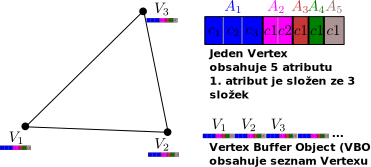
\includegraphics[width=10cm,keepaspectratio]{pics/model/primitive.pdf}
	\end{figure}
\end{frame}


